\documentclass[serif,mathserif,professionalfonts]{beamer}
\usepackage{pxfonts}
\usepackage[euler-hat-accent]{eulervm}

\usepackage{array}
\usepackage{graphicx}
\usepackage{booktabs}
\usepackage{listings}
\usepackage{fancyvrb}

\graphicspath{{.}}


\def\E{\mathop{\rm E\,\!}\nolimits}
\def\Var{\mathop{\rm Var}\nolimits}
\def\Pr{\mathop{\rm Pr\,\!}\nolimits}

\title{Statistics Primer II}
\author{David H. Alexander}
\date{August 17, 2010}

\mode<presentation>
%\usetheme{Boadilla}


% this is needed for bibliographies to work with beamer
\def\newblock{\hskip .11em plus .33em minus .07em}


\begin{document}
\setlength{\parskip}{10pt plus 1pt minus 1pt}

\maketitle

\begin{frame}{Overview}
\begin{itemize}
\item Contingency tables (categorical data)
\item Methods of evaluating significance
 \begin{itemize}
 \item Large-sample tests
 \item Exact tests
 \item Permutation tests
\end{itemize}
\item Trend tests (ordinal data)
\item Linear regression (continuous data)
\end{itemize}

\end{frame}

\section{Contingency tables}

\begin{frame}{Contingency tables}

  A contingency table allows us to cross-classify a categorical
  outcome and (one or more) categorical factors.  A $2 \times 2$
  two-way classification example:

\vspace{-0.3cm}
\begin{center}
\begin{tabular}{lccc}
                  & \multicolumn{2}{c}{Myocardial infarction} &          \\
                          \cmidrule{2-3}                             
           &        Yes       &               No                & Total  \\  \midrule  
Aspirin    &        104       &             10,933              & 11,037 \\  
Placebo    &        189       &             10,845              & 11,034 \\ \midrule
Total:     &        293       &             21,778              & 22,071  
\end{tabular}
\end{center}

In an $I \times J$ two-way classification table, factor has $I$
\emph{levels}, outcome has $J$ levels. If $J=2$, a \emph{binary}
outcome.

\end{frame}


\begin{frame}{Contingency table cell counts}
Cell counts (\emph{frequencies}) denoted $\{n_{ij}\}$.

\vspace{-0.3cm}
\begin{center}
\small
\begin{tabular}{lccc}
                  & \multicolumn{2}{c}{Outcome} &          \\
                          \cmidrule{2-3}                             
           &         +        &               -                  & Total  \\  \midrule  
Treatment  &       $n_{11}$    &            $n_{12}$              & $n_{1+}$\\
Control    &       $n_{21}$    &            $n_{22}$              & $n_{2+}$\\  \midrule 
Total:     &       $n_{+1}$    &            $n_{+2}$              & $n$
\end{tabular}
\end{center}

$n_{ij}$ generated from joint probability model $\pi_{ij}$ or from a
(conditional) \emph{success probability} $\pi_i$ for each row.  Depends on
sampling scheme.
\end{frame}


\begin{frame}{Odds ratio}
\begin{align*}
    OR \quad \doteq& \quad \frac{{\rm Odds}_{\rm \, treatment}}
                                    {{\rm Odds}_{\rm \, control}} 
    \quad = \quad \frac{\pi_{1}/(1-\pi_{1})}
                  {\pi_{2}/(1-\pi_{2})} \\[0.4cm]
   \widehat{OR}\quad \doteq& \quad  
     \frac{p_{1}/(1-p_{1})}
          {p_{2}/(1-p_{2})}, \quad \text{ where } p_1 \doteq
          n_{11}/n_{1+}, \text{ etc. } \\[0.3cm]
          \quad =& \quad \frac{n_{11} n_{22}}{n_{12} n_{21}}
 \end{align*}
\vspace{-0.5cm}
\begin{block}{Interpretation for disease studies:}
  \vspace{-0.5cm}
   \begin{itemize}
   \item $OR=1$: treatment factor and outcome are independent
   \item $OR<1$: odds of disease smaller under treatment
   \item $OR>1$: odds of disease greater under treatment
  \end{itemize}
\end{block}

\end{frame}

\begin{frame}{Does aspirin help?}
  Does taking aspirin make it more or less likely you will have a
  heart attack?

  \begin{align*}
    \widehat{OR} = \frac{(104)(10,845)}{(10,933)(189)}=0.546
  \end{align*}

  So there is some evidence associating aspirin treatment and
  decreased odds of a heart attack.

  But is there \emph{enough} evidence to make the conclusion?  i.e. is the
  observed relationship significant?

\end{frame}



\section{Evaluating significance}
\begin{frame}{Evaluating significance}
  Is there a significant association between levels of the factor, and
  the outcome?
  
  Test the null hypothesis of \emph{independence} between the factor
  and the outcome. 
\begin{align*}
  H_0&: \pi_{ij} = \pi_{i+} \pi_{+j} \\
  H_a&: \pi_{ij} \text{ unconstrained (but rows, columns must sum to one)}
\end{align*}

How can we perform the test?
\end{frame}

\subsection{Large-sample tests}

\begin{frame}{A large-sample test: Pearson's $\chi^2$}
  \begin{align*}
  X^2 & = \sum_{i,j} \frac{(n_{ij}-\hat{\mu}_{ij})^2}{\hat{\mu}_{ij}} \\
\intertext{where $\{\hat{\mu}_{ij}\}$ are estimates of the expected
          cell counts under $H_0$,} 
  \hat{\mu}_{ij} & \doteq  n p_{i+} p_{+j} = \frac{n_{i+}n_{+j}}{n}
  \end{align*}

  Asymptotically, follows a $\chi^2$ distribution with $(I-1)(J-1)$
  degrees of freedom.

  Aspirin example: $X^2=25.01$, $df=1$ $\implies p=5.7e-07$

\end{frame}

\begin{frame}{The (potential) problem with using a large sample test}
  The distribution of the test statistic $X^2$ is only close to
  the $\chi^2$ distribution for sufficiently large sample size.

  Rule of thumb: $\chi^2$ test should only be trusted to yield
  reliable results (p values) when all $\hat{\mu}_{ij} \geq 5$.
\end{frame}


\subsection{Exact tests}

\begin{frame}{Exact tests}
  Fortunately, when the sample is small, we can readily compute the
  \emph{exact} p value, not relying on any distributional
  approximations on $X^2$.

  How: compute the total probability, under $H_0$, of all
  configurations that retain the same marginal totals as observed
  table, while achieving a value of the $X^2$ statistic larger than
  that observed.
\end{frame}

\begin{frame}{Fisher's exact test}
  For the $2 \times 2$ case, this is called \emph{Fisher's exact
    test}.  Since totals fixed, $n_{11}$ determines all other entries,
  and the probability of any configuration $n_{11}$ can be written as
  \begin{align*}
     P(n_{11}) = 
      \frac{\dbinom{n_{1+}}{n_{11}} \dbinom{n_{2+}}{n_{+1}-n_{11}}} 
           {\dbinom{n}{n_{+1}}},
  \end{align*}
  a \emph{hypergeometric} probability.

 The sum of the appropriate probabilities is computed by software (R, MENDEL).
\end{frame}


\subsection{Permutation tests}

\begin{frame}{Permutation tests}

  {\bf General} mechanism for calculating the significance level of
  observed data.  Not limited to contingency tables.  Very useful when
  the distribution of the test statistic is complicated or unknown.

  Case/control association example: for each individual $i$ we have
  measured factors/covariates ${\bf x}_i$ and observed outcome $y_i$.

  Randomly permute the outcome vector ${\bf y}=\{y_i\}$ and recompute
  the measure of association (e.g. the $\chi^2$ statistic) as $X_*^2$.

  Repeat this procedure $B$ times ($B$ is large).

  $$\text{Permutation p value} = 
  \frac{ \# \text{ of times } X_*^2 \geq X^2}{B}
  $$
\end{frame}


\begin{frame}{Permutation test vs. exact test}

  Both are nonparametric alternatives to large-sample tests.

  Exact tests require enumerating \emph{all} configurations that are
  at least as favorable to $H_a$ as the observed data.  Useful when
  sample size is small.
  
  Permutation tests require enumerating a large number $B$ of
  configurations.  p value is inexact---a \emph{Monte Carlo} estimate
  of the true p value.  Useful in general situations where, for
  example, the distribution of the test statistic is complicated or
  unknown.

\end{frame}


\section{Ordinal data and trend tests}

\begin{frame}{Ordinal data and trend tests}
  Sometimes we have a categorical factor whose levels have an implicit
  ordering, i.e.
     \begin{itemize}
       \item 0 drinks/day $<$ 1-2 drinks/day $<$ 3-5 drinks/day
       \item dd $<$ Dd $<$ DD
     \end{itemize}
  An \emph{ordinal} factor.  If we assign a \emph{score} to each
  factor level, we can perform a \emph{trend test} which has
  fewer degrees of freedom than the simple $\chi^2$ test of
  independence and can thus be more powerful.

  The test statistic is the squared Pearson correlation between the
  factor score and the outcome.
\end{frame}


\begin{frame}{Cochran-Armitage trend test}
  When outcome is binary, this is called the \emph{Cochran-Armitage
    trend test}.

  Used in the additive model of genetic penetrance: 
  $$ {\sf Score}(Dd) = \tfrac{1}{2} \big[{\sf Score}(dd)+ {\sf
    Score}(DD)\big]$$

  \begin{columns}[c]
    \column{2in}
    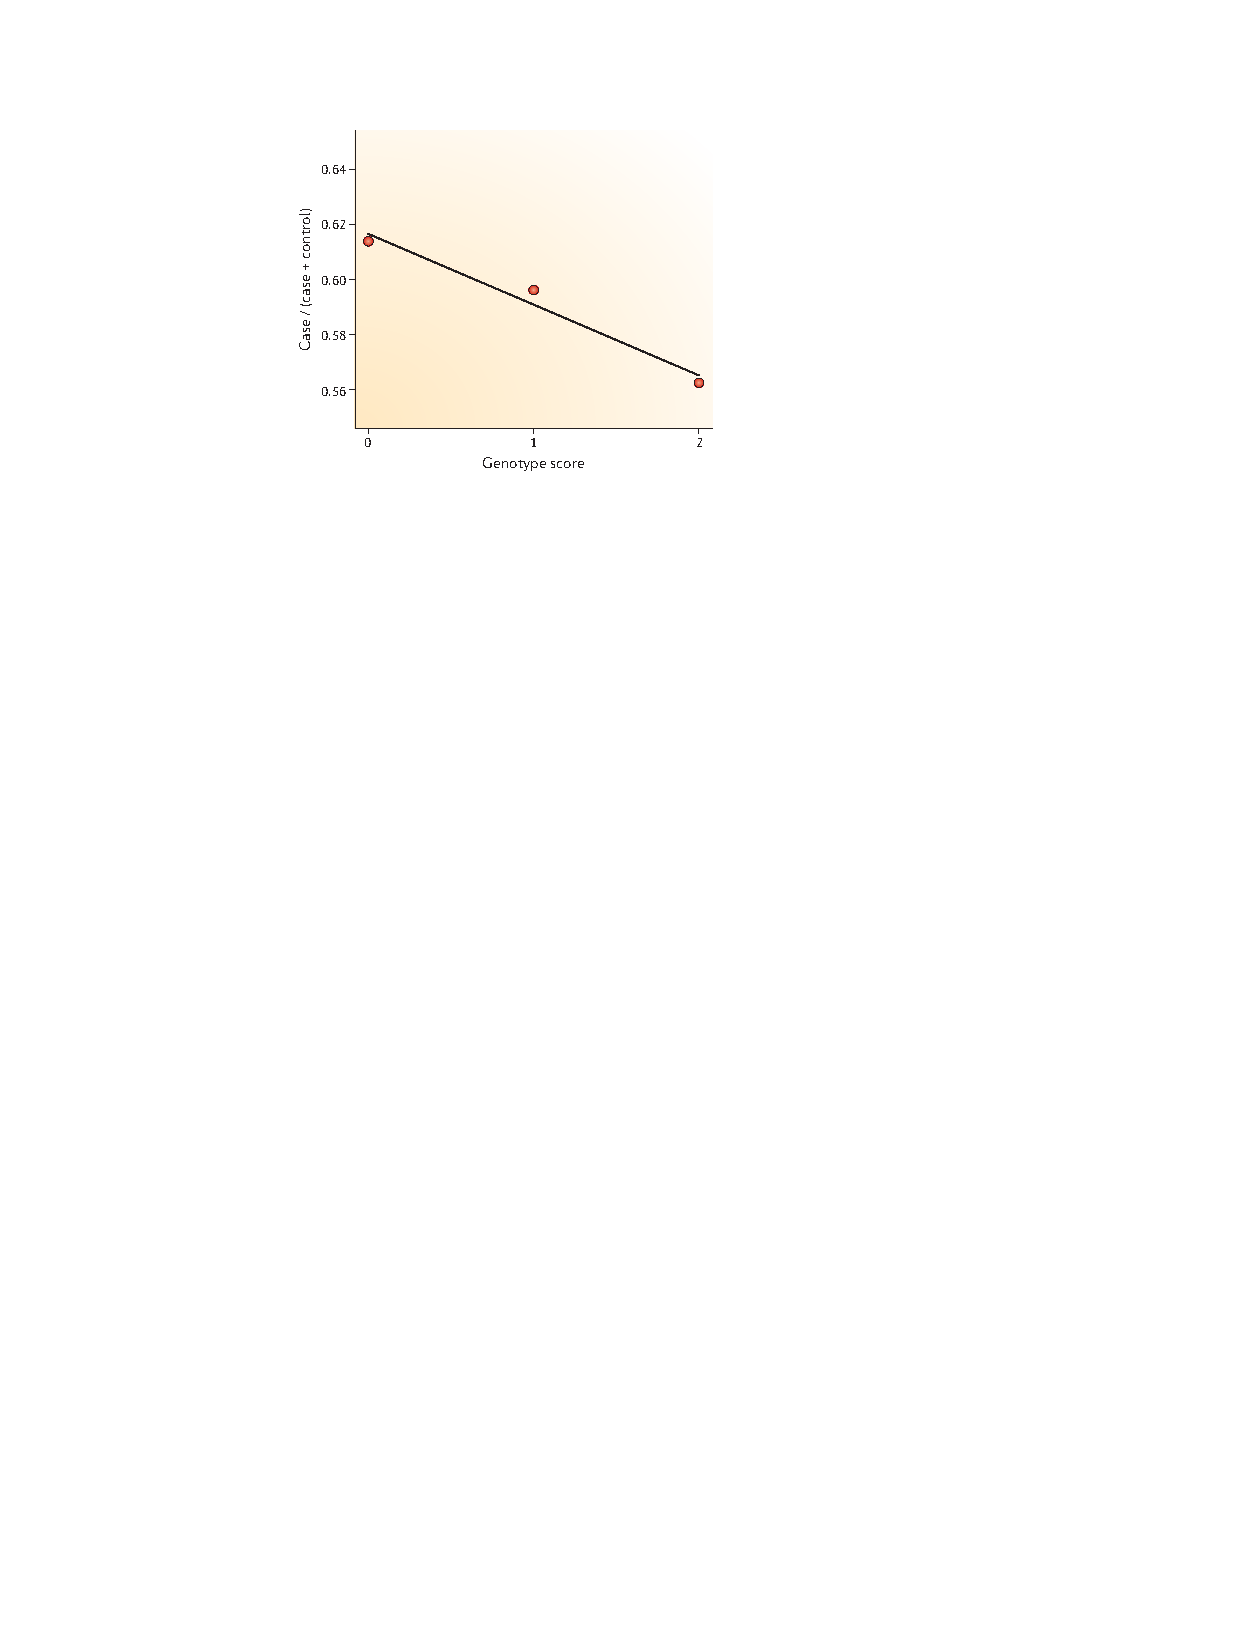
\includegraphics[width=2in]{balding-armitage.pdf}
   \column{2in}
    Testing if slope of line is zero.\\ \bigskip
    For genotypes, $df=1$, versus $df=2$ for more general $\chi^2$ test.
  \end{columns}
  \color{gray}{\small Figure credit: Balding reference}
\end{frame}

\section{Continuous data and linear regression}

\begin{frame}{Linear regression}

  \emph{Linear regression} models a linear relationship between a
  \emph{continuous} variable $X$ and a \emph{continuous} outcome $Y$.

  For example, could be used to model the relationship between height
  and weight, or the relationship between blood LDL and HDL lipid
  levels.

  $$y_i = \mu + \beta x_i + \epsilon_i$$
 
\end{frame}


\begin{frame}{Linear regression inference}
  \begin{block}{Effect size and direction}
    $$\hat{\beta} \doteq \frac
    {\sum_i (y_i-\bar{y})(x_i-\bar{x})}
    {\sum_i (x_i-\bar{x})^2}$$
   yields the \emph{least squares line} minimizing 
   \begin{align*}   
     SSE=\sum_i e_i^2, \quad \text{where }
     e_i & = y_i-\big(\hat{\mu}+\hat{\beta}x_i\big) \\[-0.3cm]
         & = y_i-\hat{y}_i
  \end{align*}
  \end{block}
  \vspace{-1cm}
  \begin{block}{Significance}
    We often want to test a simple hypothesis like $H_0: \beta=0$.
    Use a $t$-test in this case.  More complicated tests in the
    multivariate case use $F$-tests.
  \end{block}

\end{frame}


\begin{frame}{Nonlinear relationships and transformations}
  If the true relationship is nonlinear, can still use
  linear regression after \emph{transforming} $X$ or $Y$.

  \begin{columns}[c]
    \column{2in}
    \begin{center}
      $Y$ vs.$ X$
      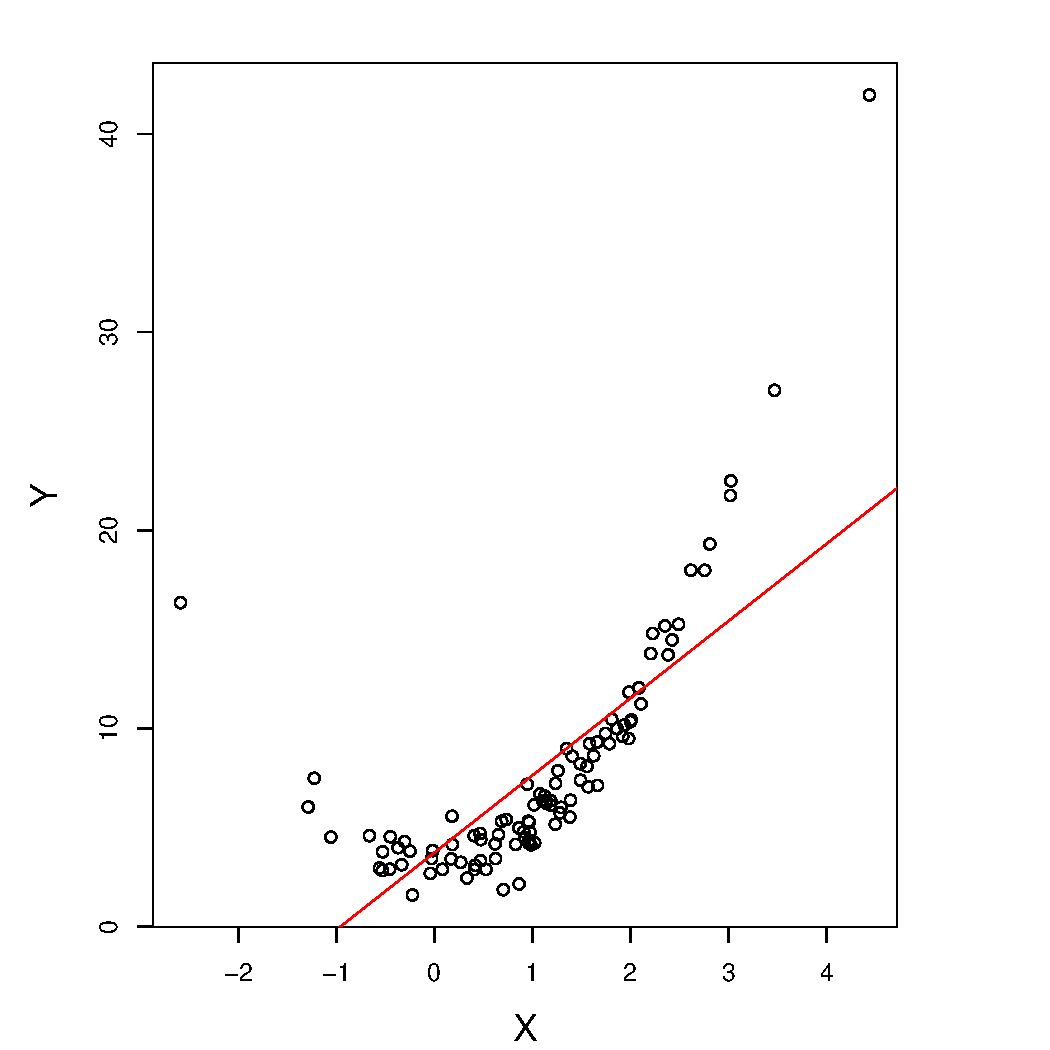
\includegraphics[width=2in]{before.pdf}
    \end{center}
   
    \column{2in}
    \begin{center}
      $Y$ vs. $X^2$
    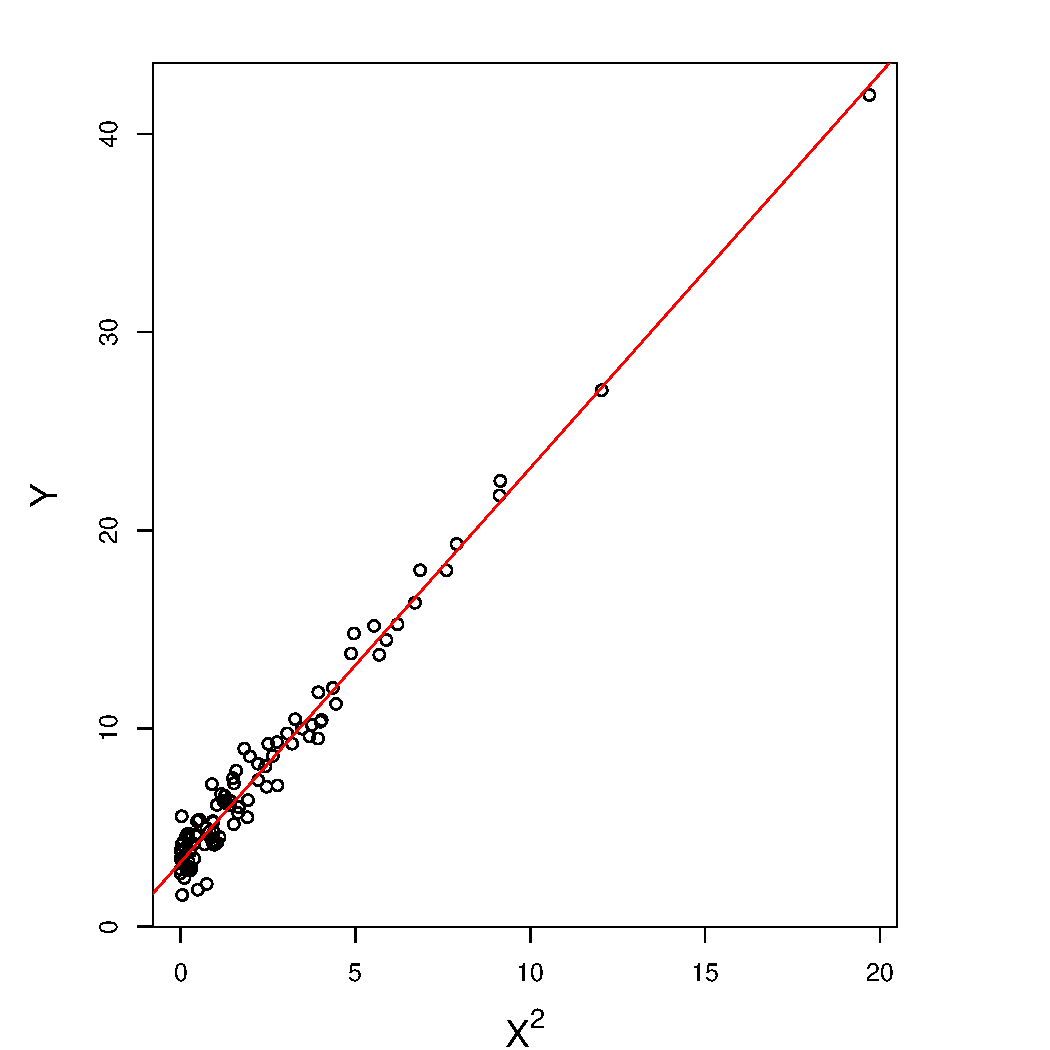
\includegraphics[width=2in]{after.pdf}    
    \end{center}

  \end{columns}

  Transformations often tried: $\log$, powers.  Search can be
  automated (e.g. Box-Cox transform).

\end{frame}



\begin{frame}{Recommended reading}
  \nocite{*}
  \bibliography{lecture-12}{}
  \bibliographystyle{unsrt}
\end{frame}



\end{document}